% -*-coding: utf-8;-*-
%%%%%%%%%%%%%%%%%%%%%%%%%%%%%%%%%%%%%%%%%%%%%%%%%%%%%%%%%%%%%%%%%
% Глава 2 - Замена линейного регулятора на нейросетевой

Подходы линейной теории автоматического регулирования широко
применяются на практике в самых различных областях.  Во многих случаях
использование линейных регуляторов и моделей объектов управления
позволяет достичь необходимого качества систем управления.  Однако по
мере совершенствования науки и техники, всё более актуальным
становятся задачи нелинейного управления.  В частности, это связано
как с повышением требований к качеству управления, когда учет
нелинейных свойств выходит на первый план, так и с рассмотрением новых
задач, решение которых с помощью линейной теории управления оказвается
невозможным.  Искусственные нейронные сети являются одним из
современных подходов, позволяющих реализовать нелинейное управление в
технических системах.

% О достоинствах (в 1-й главе):
% - неаналитичность решения
% - теоретически неограниченная мощность
% - нетребовательность к ресурсам (в режиме работы, а не обучения)
% - и пр.

Представляется актуальным разработать методику замены линейного
регулятора на нейросетевой, рассмотрев задачи выбора архитектуры
нейросети, а также выявить факторы, влияющие на качество имитации
исходного регулятора.

%TODO
%Следует также систематически сравнить
%нейросетевой регулятор с исходным линейным и выяснить их взаимные
%особенности.

Перечисленные вопросы слабо освещаются в публикациях.  В то же время,
их важность трудно оспорить --- применение любой альтернативной
парадигмы (и нейронных сетей в том числе) без понимания её свойств и
разработанной методической базы представляется ненаучным и чреватым
неожиданными проблемами в инженерной практике.

\section{Постановка задачи}

Рассмотрим систему автоматического регулирования (САР) с обратной
связью, изображенную на \figref{fig:ctrlloop}.  Будем считать, что
состояние объекта непосредственно измеряется на выходе, однако в
канале наблюдения присутствует аддитивная помеха $n(t)$ с некоторыми
постоянными свойствами.  Параметры объекта управления также постоянны
во времени.  В системе имеется линейный регулятор, поддерживающий
состояние объекта близким к заданной траектории $r(t)$.

\begin{figure}[h]
  \centering
  \input{rawctrlloop.eps_t}
  \caption{Исходная система управления.}
  \label{fig:ctrlloop}
\end{figure}

Решим задачу синтеза нейросетевого регулятора (НС--Р) для замены
имеющегося в описанной системе.  В качестве примера исходного возьмем
ПИД регулятор как наиболее типичный и распространенный в промышленных
системах автоматического регулирования.  Считая, что исходный
регулятор обеспечивает устойчивость и некоторое удовлетворительное
качество управления, можно ожидать, что достаточно точный имитатор
будет управлять системой подобно.  Качество обучения искусственной
нейронной сети определяется выбором архитектуры, обучающих данных и
параметров методики обучения.  Исследуем влияние перечисленных
факторов в задаче имитации исходного регулятора.

Будем рассматривать систему управления и её составные части в
дискретном времени с постоянным шагом дискретизации, достаточно малым,
чтобы охватить всю значимую для данной системы полосу частот.  Данный
подход позволяет моделировать саму САР и нейронные сети на компьютере.

% Архитектура НС-Р (структура входов, количество нейронов)
% Обучающая выборка (критерий достаточности объема, влияние вида выборки на качество обучения)
%TODO
% Сравнение НС-Р и ПИД (статическая ошибка, быстродействие, частотная характеристика)

%\section{Методика синтеза}???

Представим действие исходного линейного регулятора с
\figref{fig:ctrlloop} по управлению объектом как функцию $f(.)$:
\begin{equation}\label{eq:raw_controller}
  u_k=f(e_k,\mathbf{s})
\end{equation}

\noindent где $\mathbf{s}$ --- внутреннее состояние регулятора
(``память''), изменяющееся каждый такт времени по некоторому правилу.
Нейросетевой регулятор $\NN^p(.)$ должен обеспечить имитацию $f(.)$
физически реализуемым способом.  Используя квадратичный критерий,
задача синтеза НС--Р представляется в виде:
\begin{equation}\label{eq:nnp_synthesis_task}
  \sum\limits_k\big(f(e_k,\mathbf{s})-\NN^p(\mathbf{i}_k)\big)^2\rightarrow\min
\end{equation}

\noindent где $\mathbf{i_k}$ --- некоторая информация, доступная о
системе управления к моменту времени $t_k$, что определяет условие
физической реализуемости.  Способ формирования вектора $\mathbf{i}_k$,
необходимого для имитации исходного регулятора нейронной сетью,
является отдельной задачей, которую необходимо решить.

Сформулированная задача эквивалентна общей задаче нейросетевой
аппроксимации неизвестной фунции $f(.)$, заданной таблично
(см.~\eqref{eq:supervised_learning_task}) с помощью нейронной сети
$\NN(.)$.  В известной работе \cite{rumelhart86} был предложено
обобщенное дельта-правило ({\em generalized delta-rule}) для обратного
распространения ошибки в многослойном персептроне, решающее эту
задачу.  Было теоретически доказано~\cite{XXX}\marginpar{где?}
существование такой функции $\NN(.)$.

Таким образом, задача синтеза НС--Р распадается на следующие
подзадачи:
\begin{enumerate}
\item Выбор архитектуры НС--Р, в том числе, вектора информации о
  системе $\mathbf{i}_k$.
\item Сбор обучающих данных.
\item Собственно обучение НС--Р методом обратного распространения
  ошибки.
\end{enumerate}

Третья подзадача решается общеизвестным способом
(см. п.~\ref{nn_learning_algorithms}).  Рассмотрим первые две
подзадачи.

\section{Архитектура нейросетевого регулятора}

ПИД регулятор представляет собой динамическую систему, обладающую
памятью (кроме простейшего случая пропорционального управления).  Для
адекватной имитации нейронная сеть регулятора также должна обладать
динамическими свойствами.  При синтезе нейросетевой модели объекта
управления (см. п.~\ref{identif_and_nnp}), эта задача решается либо за
счет добавления обратных связей, либо за счет организации внешней
памяти в виде элементов задержки.

Сравнивая задачу обучения НС--Р с задачей синтеза нейросетевой модели
объекта следует при очевидном сходстве (имитация некоторой линейной
системы) отметить два фундаментальный различия.  Во-первых, НС--О
может быть реализована как в виде автономной модели поведения, так и в
виде зависимой от объекта модели предсказания, в то время как НС--Р
должен полностью заменить исходный регулятор.  Во-вторых, назначение
НС--О --- копирование поведения объекта управления, а НС--Р должен
быть сначала обучен подобно исходному линейному регулятору, но потом,
в соответствии с заданными правилами (например, минимизация
среднеквадратической ошибки или подстройка под нестационарный объект),
может изменить свои свойства.  Буквальное повторение свойств исходного
линейного регулятора не является самоцелью, а лишь позволяет
сопоставить нейросетевой и традиционный линейный регуляторы.  По этой
причине не имеет смысла формировать архитектуру нейросетевого
регулятора базируясь на свойстве линейности исходного.

Как и в случае с синтезом НС--О возникает задача выбора между
статической и динамической (с обратными связями) архитектурами
нейронной сети.  Аргументом в пользу динамической нейронной сети
является наиболее очевидный путь имитации свойств линейной
динамической системы с помощью автономной модели.  Вместе с тем, у
динамической нейронной сети имеются как недостатки общего плана,
упомянутые в п.~\ref{identif_and_nnp}, так и специфические,
проявляющиеся при использовании обратных связей в НС--Р:

\begin{enumerate}
\item эффект исчезающего градиента при обучении по методу BPTT;
\item увеличение требований к ресурсам и усложнение алгоритма обучения
      в контуре, вызванное процедурой обращения времени;
\item усложнение анализа устойчивости системы за счет появления еще
      одного контура обратной связи с нелинейным элементом (нейросетью).
\end{enumerate}

Применение статической нейронной сети для реализации НС--Р не имеет
перечисленных недостатков, кроме того, обучение статической нейросети
в целом осуществляется быстрее, чем динамической.  Однако, как и в
случае с нейросетевой моделью объекта управления, следует с помощью
надлежащего формирования структуры входов нейросети обеспечить
динамические свойства НС--Р, аналогичные имеющимся у ПИД регулятора в
контуре.

\subsection{Структура входов нейросети}\label{nnc_inputs}

Рассмотрим несколько вариантов формирования вектора входных значений
$\mathbf{i}_k$ для НС--Р (см. \eqref{eq:nnp_synthesis_task}).
Обязательно следует проверить вариант подключения, аналогичный
исходному регулятору.  В этом случае на вход подается только значение
ошибки в текущий момент времени $e_k$.  Как было показано ранее при
построении нейросетевой модели объекта, этот вариант подключения
статической нейронной сети не может обеспечить адекватную имитацию
свойств динамической системы.  Чтобы преодолеть ограничение
статического отображения надо искусственно организовать память с
помощью повторения прошлых входов $e_k\ldots e_{k-d}$.  Поэтому
исследуем поведение НС--Р при различных значениях емкости памяти:
$0\le d\le 4$.

Рассмотрим также варианты подключения НС--Р с входами $e_k,\Delta e_k$
и $r_k,e_k$.  Первый вариант обеспечивает нейросеть информацией о
динамике с помощью дискретной производной сигнала ошибки управления, а
второй представляет собой объединение концепций управления по
возмущению $r(t)$ и отклонению $e(t)$.

Для сравнения перечисленных вариантов формирования входного вектора
НС--Р была проведена серия экспериментов.  Ниже приводится постановка
и результаты одного из них.

% nn/dpid.new/contrp/...
Эксперимент проводился в условиях стохастической уставки при наличии
случайной аддитивной помехи в наблюдаемом выходе объекта управления.
Формирующие фильтры уставки $R^*(z)=\frac{0.625z}{z-0.779}$ и помехи
$N^*(z)=0.4$.  Объект $P^*(z)=\frac{z}{z-0.5}$ управлялся ПИД
регулятором $C^*(z)=0.4 + 0.5\frac{z}{z-1} +
0.05\frac{z^2-2z+1}{z(z-1)}$.  Регулятор был настроен на ступенчатом
возмущающем сигнале по критерию минимизации длительности переходного
процесса при максимальном перерегулировании в пределах 4\% амплитуды
возмущающего сигнала.

Нейронная сеть регулятора имела архитектуру $\NN^p_{x,7,3,1}$,
где $x$ --- размерность входного вектора.  Обучение осуществлялось на
выборке длиной 200 в течение 400 эпох, а контрольная выборка имела
длину 500, причем если ошибка на контрольной выборке начинала
возрастать, то обучение досрочно прекращалось.  Критерием обучения
являлась минимизация среднеквадратичной ошибки воспроизведения.

\begin{table}[ht]
\centering
\caption{Сравнение точности имитации ПИД регулятора вне контура управления
         при различном способе формирования входного вектора НС--Р и
         различных параметрах уставки и помехи}
\label{tabl:nnc_pretr_input_vec}
\begin{tabular}{|c|l|c|c|c|c|}
\hline
\multicolumn{2}{|r|}{Эксперимент} & {\sf А} & {\sf Б} & {\sf В} & {\sf Г}\\
\hline
\multicolumn{2}{|r|}{Уставка} &
  \multicolumn{2}{|c|}{Стохастическая $R^*(z)$} & $\sin(t)$ & $0$ \\
\hline
\multicolumn{2}{|r|}{Помеха} & $N^*(z)=0.4$ & $N^*(z)=0.7$ & $N^*(z)=0.4$ & $N^*(z)=0.4$\\
\hline\hline
N   & Входной               & \multicolumn{4}{|c|}{Среднеквадратическая ошибка} \\
пп. & вектор $\mathbf{i}_k$ & \multicolumn{4}{|c|}{на контрольной выборке}\\
\hline
1 & $e_k$                 & 0.3228 & 0.2906 & 0.1299 & 0.0027\\
2 & $e_k,e_{k-1}$         & 0.2993 & 0.2710 & 0.1291 & 0.0022\\
3 & $e_k\ldots e_{k-2}$   & 0.2709 & 0.2459 & 0.1270 & 0.0016\\
4 & $e_k\ldots e_{k-3}$   & 0.2482 & 0.2284 & 0.1240 & 0.0013\\
5 & $e_k\ldots e_{k-4}$   & 0.2385 & 0.2163 & 0.1188 & 0.0013\\
6 & $e_k,\Delta e_k$      & 0.2980 & 0.2738 & 0.1293 & 0.0023\\
7 & $r_k,e_k$             & 0.0388 & 0.0968 & 0.0039 & 0.0040\\
\hline
\end{tabular}
\end{table}

%% $e_k$     0.1296
%% $r_k,e_k$ 0.0037

В \tablref{tabl:nnc_pretr_input_vec} результаты эксперимента приведены
в столбце {\sf А}.  Анализ значений среднеквадратичной ошибки
показывает, что увеличение емкости памяти прошлых входов позволяет
лишь незначительно уменьшить ошибку имитации (строки таблицы 1--5).
Вариант с первой разностью ошибки (строка 6) показывает близкие
результаты с вариантом $e_k,e_{k-1}$ (строка 2).  Очевидно, что для
НС--Р эти варианты информационно эквивалентны.  Наилучшее качество
имитации исходного регулятора было достигнуто НС--Р с входным вектором
$r_k,e_k$, причем достигнутый уровень ошибки в этом случае оказался
меньше почти на порядок, чем в остальных.

Эксперименты показали, что при увеличении мощности помехи
относительное преимущество НС--Р с входным вектором $r_k,e_k$
уменьшается (столбец {\sf Б} таблицы).  Таким образом, применение в
качестве входного вектора $e_k\ldots e_{k-d}$ может оказаться в
некоторых случаях оправданным.

Были также рассмотрены случаи предварительного обучения НС--Р по
детерминированной уставке различной формы.  По результатам
экспериментов наилучшим вариантом формирования входного вектора с
большим отрывом оказалось совмещенное управление по возмущению и
отклонению: $r_k,e_k$ (строка 6).  Оказалось также, что результирующий
уровень ошибки при периодической уставке практически не зависит от ее
формы.  В частности, числовые значения среднеквадратичной ошибки на
гармоническом сигнале (столбец {\sf В}
\tablref{tabl:nnc_pretr_input_vec}) и на меандре примерно одинаковы.

Отдельно был рассмотрен случай задачи стабилизации, когда уставка
постоянна, например, равна 0 (столбец {\sf Г}
\tablref{tabl:nnc_pretr_input_vec}).  Нейросетевой регулятор с
входным вектором $r_k,e_k$ показал худший результат, чем любой из
вариантов с повторением прошлых значений ошибки.  Видно, что
отсутствие влияния уставки на нейронную сеть в данном случае делает
наличие входа $r_k$ не только бесполезным, но и вредным.

Проводились также эксперименты с объектом управления с чистым
запаздыванием и объектом управления второго порядка, анализ которых
обнаружил те же закономерности.

По результатам проведенных экспериментов можно сформулировать
некоторые рекомендации по формированию входного вектора нейросетевого
регулятора по критерию наилучшей имитации исходного ПИД регулятора:

\begin{itemize}
\item
В случае задачи стабилизации (постоянное значение уставки)
рекомендуется использовать один из вариантов с повторением прошлых
значений: $e_k\ldots e_{k-d}$.  При увеличении емкости памяти прошлых
значений (параметр $d$) качество имитации при наличии помехи будет
возрастать.

\item
В случае изменяющегося значения уставки предпочтительным является
совмещенное управление по возмущению и отклонению: $r_k,e_k$.  При
значительном уровне помехи улучшить качество имитации можно вводя и
увеличивая память прошлых состояний.  Входной вектор в этом случае
будет иметь вид $r_k,e_k\ldots e_{k-d}$
\end{itemize}

%Испытание предварительно настроенного НС--Р в системе управления
%вместо ПИД регулятора показало, что система успешно управляется
%нейросетью.  Во всех проведенных экспериментах система с нейросетевым
%регулятором в контуре не потеряла устойчивости.  Вместе с тем отмечен
%ряд особенностей и недостатков, присущих нейросетевому управлению:

%\begin{enumerate}

%\item быстродействие нейросетевого регулятора не хуже ПИД, а время
%наступления установившегося режима даже меньше, чем у ПИД регулятора
%(\figref{fig:pid_npc_test}а);

%\item при неизменной уставке (в том числе, при $r(t)=0$) в системе
%с НС--Р может иметь место статическая ошибка (на примере со
%ступенчатой уставкой на \figref{fig:pid_npc_test}а видно, что
%перерегулирование составляет 6\% номинального уровня);

%\item при выходе уровня уставки за пределы диапазона обучающих данных
%точность управления падает (\figref{fig:pid_npc_test}б).
%\end{enumerate}

%\begin{figure}[h]
%\begin{tabular}{cc}
%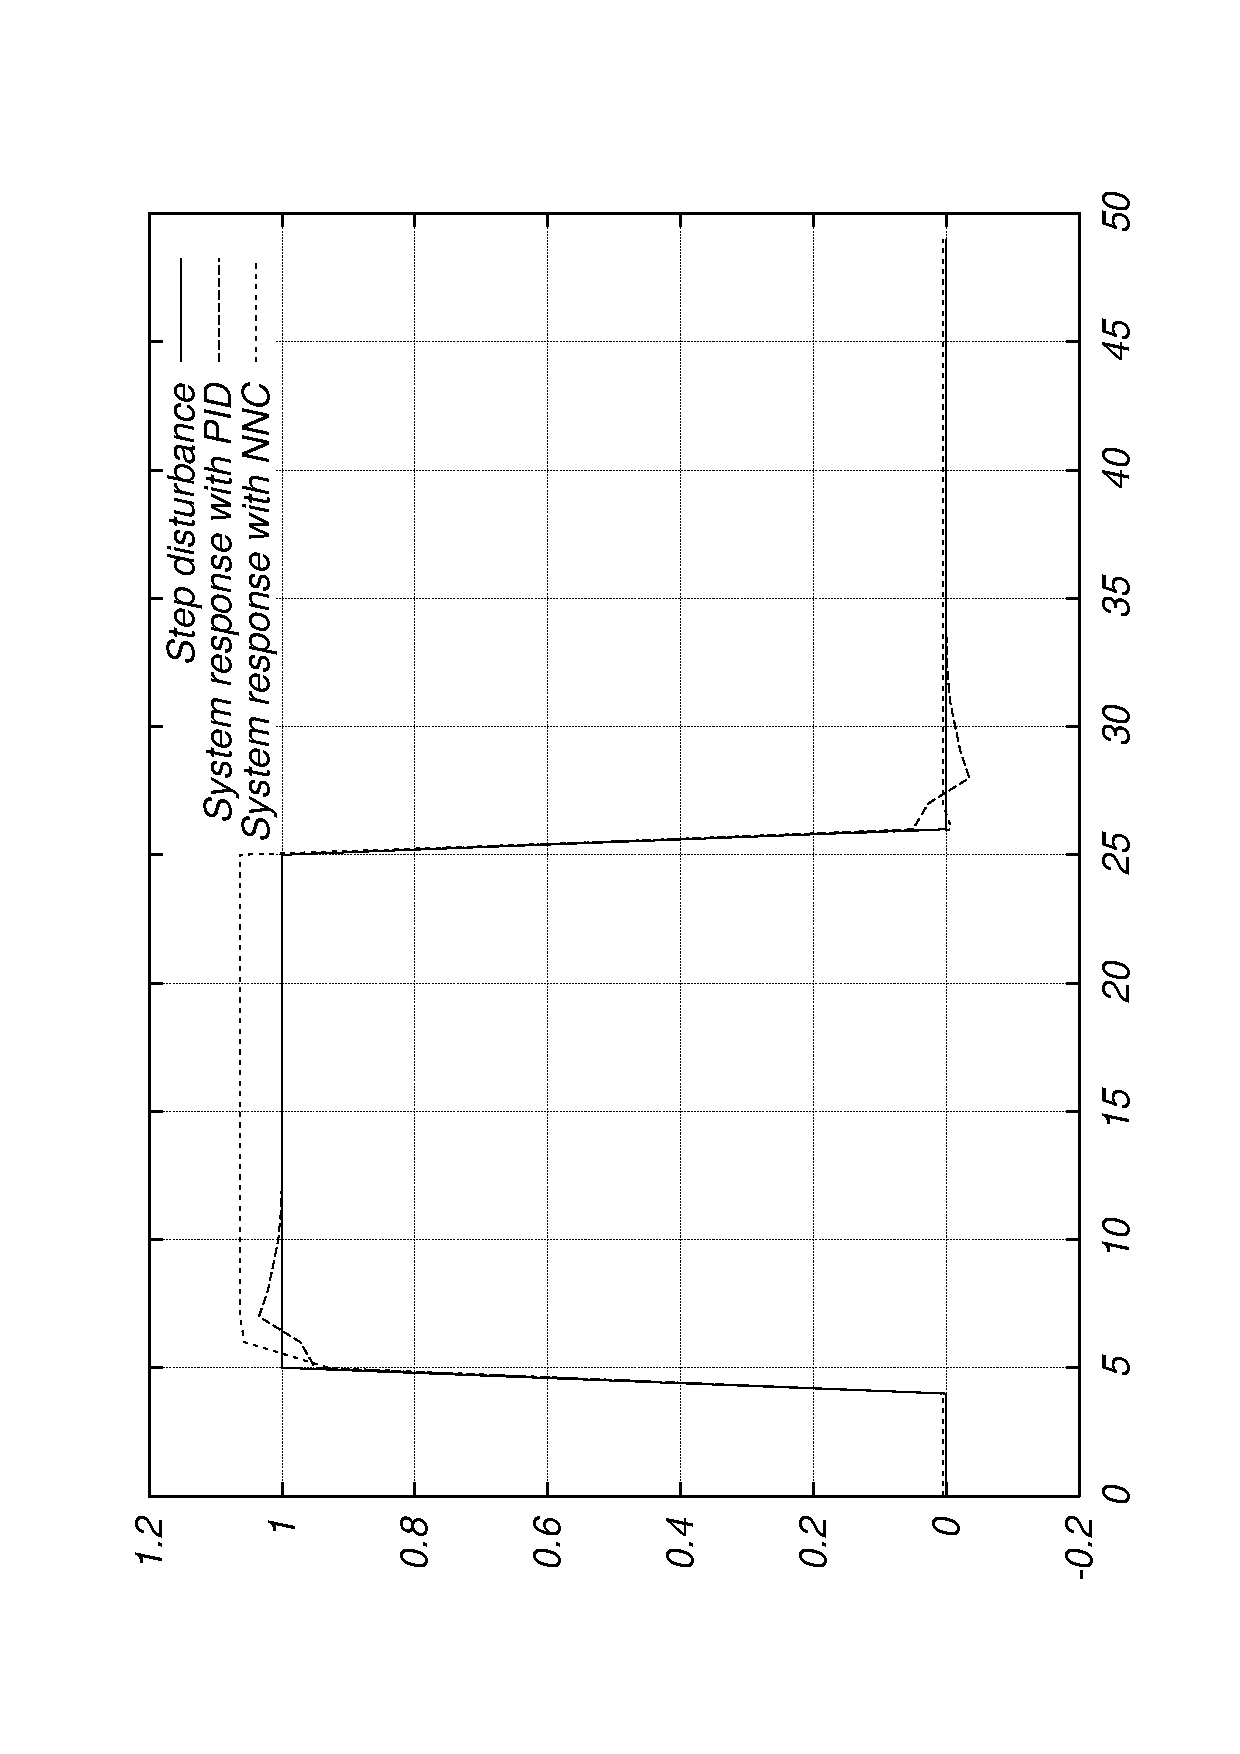
\includegraphics[angle=270,width=0.45\textwidth,%
%             totalheight=0.25\textheight]{pid_npc_step_test} &
%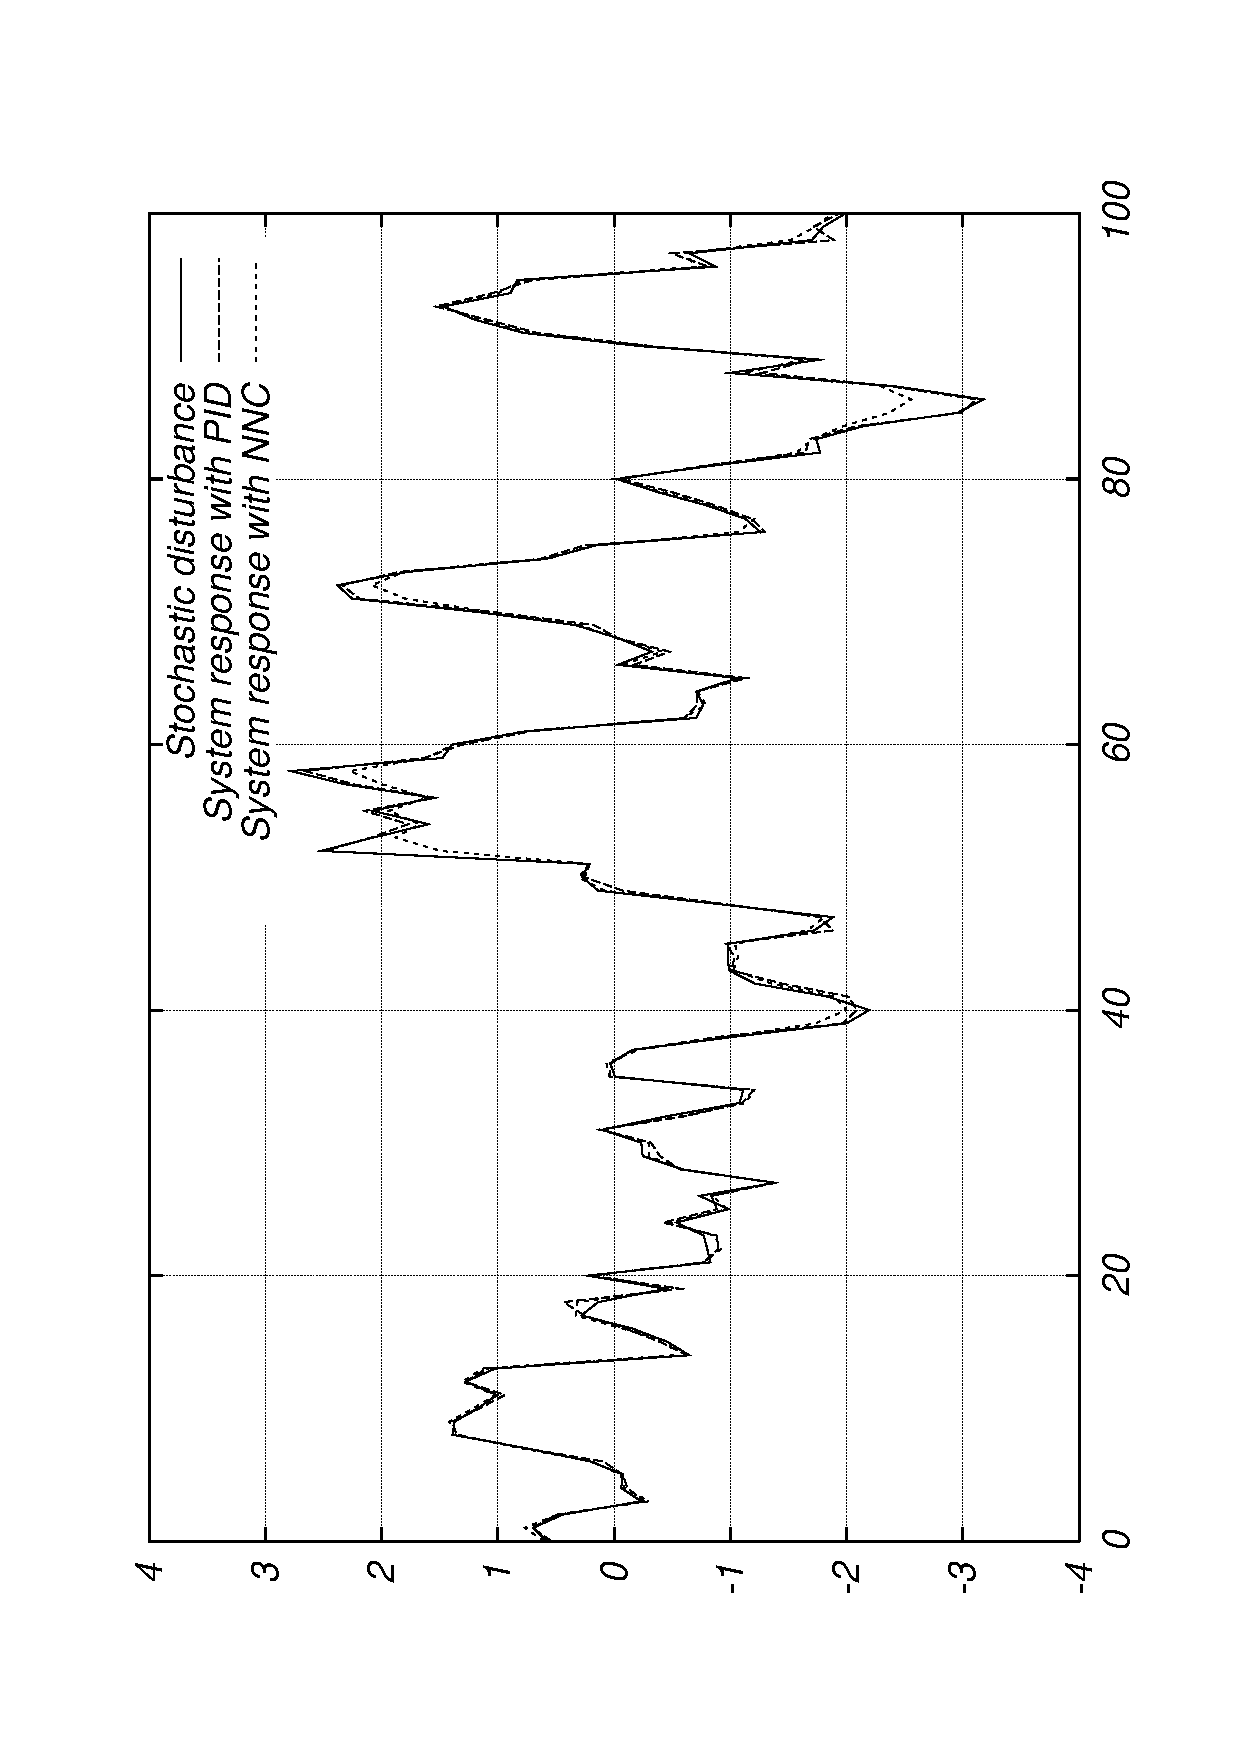
\includegraphics[angle=270,width=0.45\textwidth,%
%             totalheight=0.25\textheight]{pid_npc_stoch_test} \\
%а) & б)\\
%\end{tabular}
%\caption{Отклик системы на прямоугольное (а) и стохастическое (б)
%         возмущающее воздействие при ПИД и НС регулировании ($r_k,e_k$).}
%\label{fig:pid_npc_test}
%\end{figure}

%Рассмотрим значимость последних двух эффектов и способы их
%устранения.

%\paragraph{Статическая ошибка НС--Р}\label{nnc_static_error}
%Эффект статической ошибки был рассмотрен при обучении нейросетевой
%модели объекта управления.  Он связан с различием формы обучающего и
%контрольного сигнала.  В частности, статическая ошибка будет возникать
%на ступенчатой уставке в том случае, если нейросетевой регулятор был
%обучен на стохастическом сигнале уставки.  Эффект статической ошибки
%нейронной сети, как отмечалось на \pgref{amplify-zero}, проявляет себя
%на ступенчатом контрольном сигнале уставки усилением нуля и ошибочным
%коэффициентом передачи.  Отмечается, что для компенсации этого
%нежелательного эффекта можно использовать параллельно с нейросетевым
%линейный регулятор~\cite{steck96}.  Далее рассмотрим способы
%устранения эффекта статической ошибки, не требующие в включения в
%контур управления дополнительных узлов.

%Если условия нормальной эксплуатации регулятора в контуре управления
%характеризуются кусочно-постоянной уставкой, рекомендуется для
%настройки НС--Р взять обучающую выборку, имеющую подобный вид.  В этом
%случае нейросетевая аппроксимация поведения ПИД регулятора будет более
%качественной.  Однако полностью устранить этим способом эффект
%статической ошибки не всегда удается.

%Значительно лучший результат дает подход, основанный на предположении
%о симметрии функций $u_{PID}(t)$ при симметрии функций $r(t)$, $e(t)$
%относительно нуля (или любого другого известного постоянного среднего
%значения).  В этом случае задача аппроксимации для нейронной сети
%упрощается, так как отпадает потребность в пороге --- весовом
%коэффициенте $w_0$ (см. формулу \eqref{eq:neuron_output}), ---
%предназначенном для смещения рабочей области функции активации.
%Функционирование нейрона в этом случае определяется уравнением

%\begin{equation}\label{eq:neuron_output_nobias}
%y=\fa(\sum_{j=1}^nw_j x_j)
%\end{equation}

%После предварительного обучения НС--Р с нулевым порогом на
%стохастическом обучающем множестве контрольная проверка на единичной
%ступени показала уменьшение эффекта статической ошибки по сравнению со
%случаем использования обычных нейронов со смещением $w_0$
%(\figref{fig:npc_static_error}).  В частности, ошибка в имитации
%коэффициента передачи уменьшилась с 6\% до 4.5\%, а эффект усиления
%нуля уменьшился до исчезающе малых величин.

%\begin{figure}[h]
%\centering
%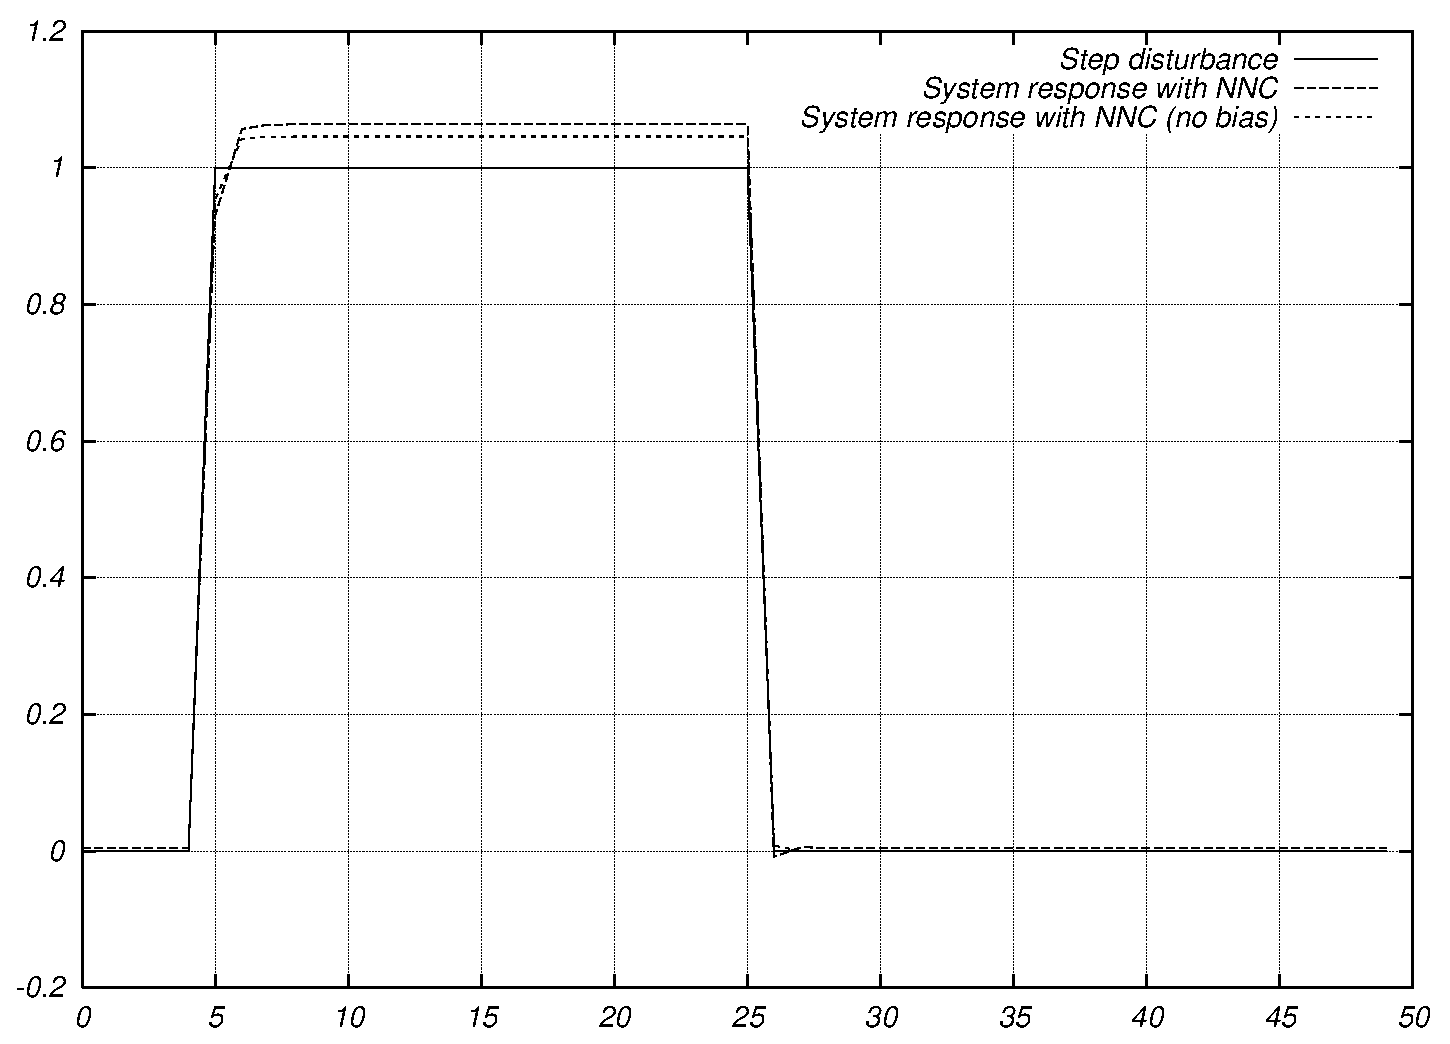
\includegraphics[angle=270,width=0.8\textwidth,%
%             totalheight=0.35\textheight]{npc_nob_step_test}
%\caption{Эффекты статической ошибки НС--Р в случаях наличия смещения $w_0$ у
%         нейронов сети и в случае его отсутствия.}
%\label{fig:npc_static_error}
%\end{figure}

%Следует отметить, что эффект статической ошибки проявляет себя в
%основном на участках постоянной уставки при полном отсутствии помех.
%В случае наличия постоянных изменений на входах НС--Р, которые могут
%быть вызваны изменениями уставки или шумом в канале наблюдения, эффект
%статической ошибки себя не проявляет.  Это означает отсутствие
%различий между исходным ПИД регулятором и предварительно обученным
%нейросетевым.  Подобным может считаться случай синтеза Винеровского
%оптимального регулятора вследствие наличия случайных помех и
%стохастической природы уставки.

\subsection{Внутренняя структура нейросети}

Исследуем влияние количества скрытых слоёв и нейронов в них на
процесс обучения и качество имитации исходного регулятора.  Для этого
возьмем несколько нейронных сетей с входами $r_k,e_k$ и количеством
скрытых слоёв от 0 до 3 и обучим их на одних и тех же данных.  В
качестве обучающего множества будем использовать выборку длиной 800
отсчетов, а в качестве контрольной --- длиной 200 отсчетов.  Обе
выборки получены при стохастической уставке и случайной помехе.

Продолжительность обучения Скорость пакетного обучения измерялась как количество эпох за которые
НС--Р достигла ошибки 0.006.  Если за 3000 эпох ошибка всё ещё была
больше заданного уровня, то обучение останавливалось на достигнутом
результате.  После обучения НС--Р включался в контур управления и в
условиях отсутствия помехи на вход системы поступала ступенчатая
уставка.  Качество управления оценивалось по среднеквадратической
ошибке управления на ступенчатой уставке.  Результаты эксперимента
приведены в \tablref{tabl:nnp_internal_arch}.

\begin{table}
\caption{Влияние внутренней структуры НС--Р на обучение и качество имитации.}\label{tabl:nnp_internal_arch}
\begin{tabular}{|l|c|c|c|c|}
\hline
$\mathrm{N}^o$ & Архитектура НС--Р & Ошибка обучения & Ошибка управления & Время вычислений, с\\
\hline
1 & $\NN^p_{r+e,1}$          & 0.0066& 0.0058 & 57.0\\
2 & $\NN^p_{r+e,5,1}$        & 0.0065& 0.0061 & 76.2\\
3 & $\NN^p_{r+e,20,1}$       & 0.0065& 0.0060 & 132.1\\
4 & $\NN^p_{r+e,7,5,1}$      & 0.0067& 0.0061 & 120.2\\
5 & $\NN^p_{r+e,20,10,1}$    & 0.0067& 0.0063 & 306.6\\
6 & $\NN^p_{r+e,7,9,5,1}$    & 0.0070& 0.0062 & 194.4\\
7 & $\NN^p_{r+e,15,20,10,1}$ & 0.0067& 0.0064 & 571.1\\
\hline
\end{tabular}
\end{table}

На основании проведенных экспериментов можно сделать вывод, что
внутренняя структура многослойного персептрона НС--Р с входами
$r_k,e_k$ не оказывает значительного влияния на качество имитации ПИД
регулятора.  В то же время, количество нейронов в нейронной сети
напрямую определяет вычислительную сложность процесса обучения.
Поэтому усложнение внутренней архитектуры НС--Р увеличивает время
вычислений.  Очевидно, в такой ситуации предпочтительнее использовать
более простые архитектуры.  Однако, следует иметь в виду, что
возможность нейросетевой аппроксимации произвольной функции доказано
только для сетей с не менее чем двумя слоями нелинейных нейронов.

\section{Обучающие данные}

Обучение искусственной нейронной сети с учителем требует наличия
набора данных, определяющих эталонные пары вход-выход.  Для
нейросетевого регулятора с комбинированным управлением по возмущению и
отклонению входом является пара $r_k,e_k$, а выходом --- управляющее
воздействие исходного регулятора $u_k$.  Эти данные легко получить при
наблюдении за функционированием системы управления.  Однако возникает
вопрос об оптимальном объёме данных, а также о наилучшем пробном
сигнале для обучения НС--Р.

\subsection{Вид пробного сигнала}

При настройке линейных регуляторов (в частности, ПИД) в контуре, как
правило, используются детерминированные сигналы уставки ступенчатой
или гармонической формы.  В то же время, в процессе работы уставка
обычно изменяется случайным образом.  Исследуем в эксперименте, какой
из перечисленных трех видов уставки обеспечивает обучение НС--Р для
наилучшей имитации исходного регулятора.  Для этого сгенерируем
временные ряды одинаковой длительности $L=2000$: меандр,
моногармонический сигнал и цветной шум (формирующая функция
$R^*(z)=\frac{0.625z}{z-0.779}$).  Фрагмент полученных рядов уставки
приведен на~\figref{fig:probe_signals}.  В числе внешних воздействий
на систему кроме уставки имеет место случайная помеха в канале
наблюдения.  В эксперименте она является нормально распределенным
белым шумом с нулевым средним и дисперсией 0.01.

\begin{figure}
\centering
\includegraphics[width=0.8\textwidth,%
  totalheight=0.35\textheight]{probe_signals_rus}
\caption{Временные ряды уставки разных видов.}\label{fig:probe_signals}
\end{figure}

По плану эксперимента уставка выбранного вида подавалась на вход
системы управления с исходным ПИД регулятором, после чего временные
ряды ошибки управления $e(t)$ и управляющего воздействия $u(t)$
сохранялись.  С их помощью осуществлялась настройка НС--Р с
архитектурой $\NN^p_{r+e,5,1}$.  Обученный НС--Р помещался на место
исходного ПИД регулятора в контур управления и на вход системы
подавалась ступенчатая уставка.  Для лучшей иллюстративности помеха в
систему не подавалась.  Наилучшее качество имитации ПИД регулятора
должно обеспечивать наилучшее качество управления: величину
перерегулирования, время затухания переходного процесса.

Результаты управления настроенных НС--Р в контуре показан
на~\figref{fig:nnc_system_response}.  Видно, что наихудшим оказался
НС--Р, настроенный на ступенчатой уставке, так как он привел к
высокочастотным осцилляциям в системе без каких-либо признаков
стабилизации состояния объекта.  НС--Р, обученный на гармонической
уставке, обеспечил управление объектом, однако величина
перерегулирования, время переходного процесса и остаточная ошибка при
постоянном уровне уставки достаточно велики.  Наилучший результат
показал НС--Р, настроенный на стохастической уставке.  При чуть
меньшем перерегулировании он обеспечил гораздо более короткий
переходный процесс и существенно меньшую остаточную ошибку.  Результат
работы этого нейросетевого регулятора в сравнении с исходным ПИД
показан на \figref{fig:nnc_pid_system_responses}.

\begin{figure}
\centering
\includegraphics[width=0.8\textwidth,%
  totalheight=0.35\textheight]{nnc_system_response_rus}
\caption{Результат работы НС--Р, настроенного на обучающих данных с уставкой
         разных видов.}\label{fig:nnc_system_response}
\end{figure}

\begin{figure}
\centering
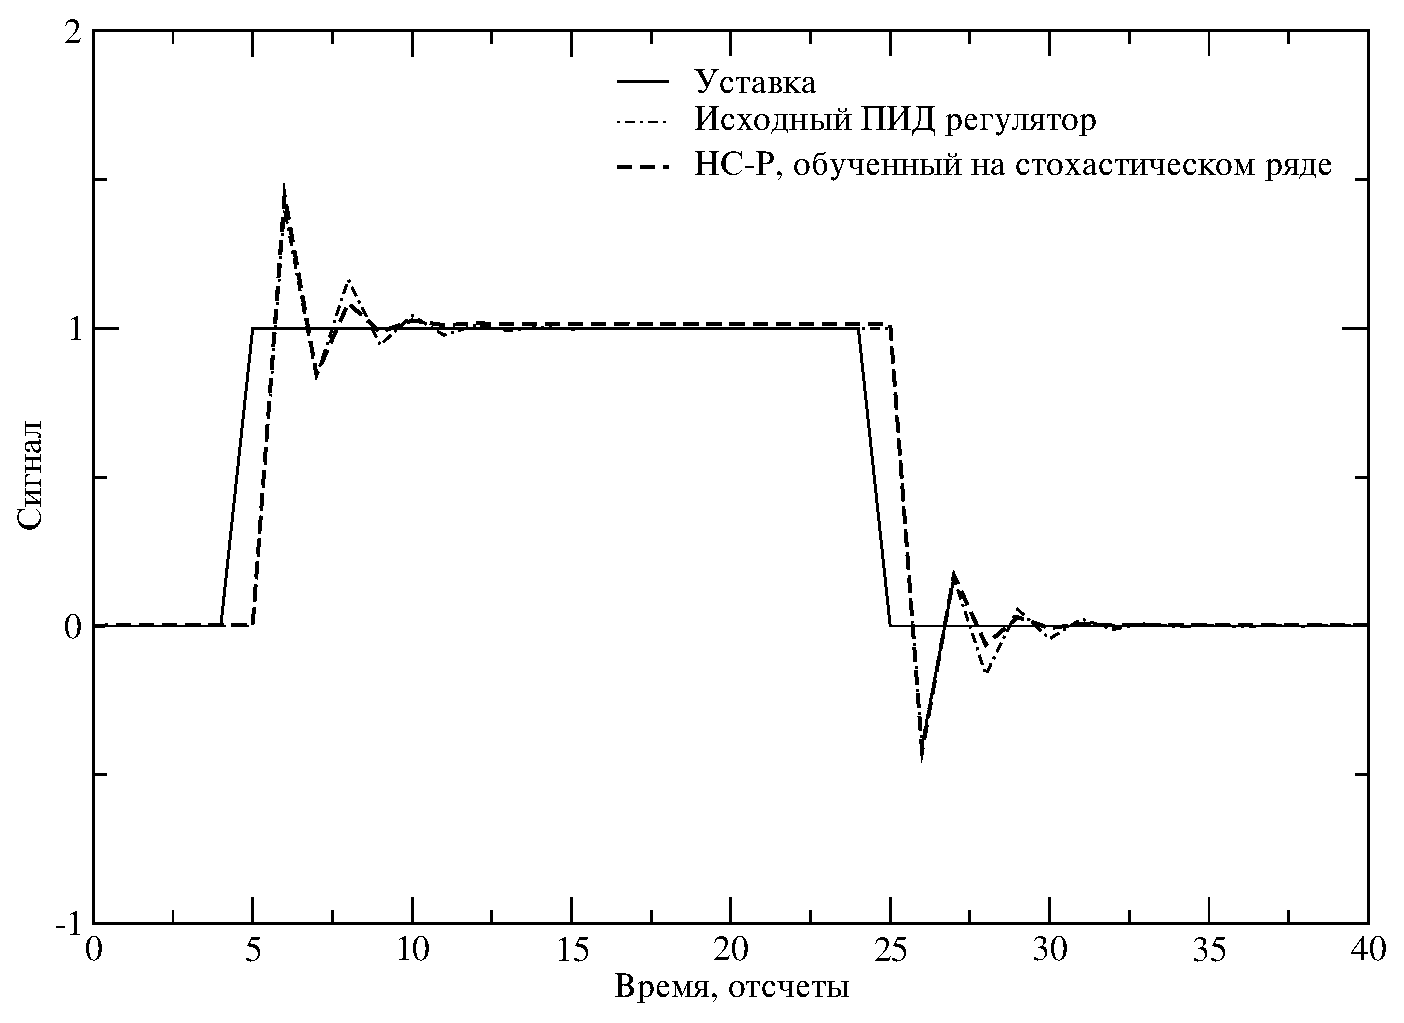
\includegraphics[width=0.8\textwidth,%
  totalheight=0.35\textheight]{nnc_pid_system_responses_rus}
\caption{Сравнение работы исходного ПИД регулятора с лучшим НС--Р.}%
\label{fig:nnc_pid_system_responses}
\end{figure}

Если для обучающей выборки целесообразно использовать стохастическую
уставку, то для контрольной выборки лучше всего взять уставку,
наиболее типичную для данной системы автоматического регулирования.

\subsection{Объём обучающих данных}

Причины значительного преимущества стохастических пробных сигналов
перед детерминированными кроются в более равномерном покрытии области
определения функции нейронной сети обучающими точками.  Для НС--Р
рассматриваемой архитектуры входное множество двумерное и оно
образуется парами $r_k,e_k$.  Плотность покрытия обучающими точками
для трех видов уставок, участвовавших в эксперименте, приводится
на~\figref{fig:probe_signals_re2d}.  Видно, что обучающие точки,
полученные при периодической ступенчатой уставке, сгруппированы на
очень малой площади.  Гармоническая уставка дает более равномерное
распределение, но её периодичность проявляется областями чрезмерной
концентрации обучающих точек, регулярно расположенных на плоскости.
Стохастическая уставка обеспечивает покрытие плоскости $r\times e$
обучающими точками по закону распределения, близкому к двумерному
нормальному.  В эксперименте получена следующая приблизительная оценка
покрытия обучающими точками рабочей части плоскости $r\times e$
(диапазон уставок $[-3,3]$, диапазон ошибок $[-2,2]$): уставка-меандр
дает 14\% покрытия, моногармоническая уставка --- 43\%, стохастическая
--- 72\%.  Очевидно, что в последнем случае обучение нейронной сети
для рабочей части плоскости будет наиболее полноценным.

\begin{figure}
\centering
\begin{tabular}{c}
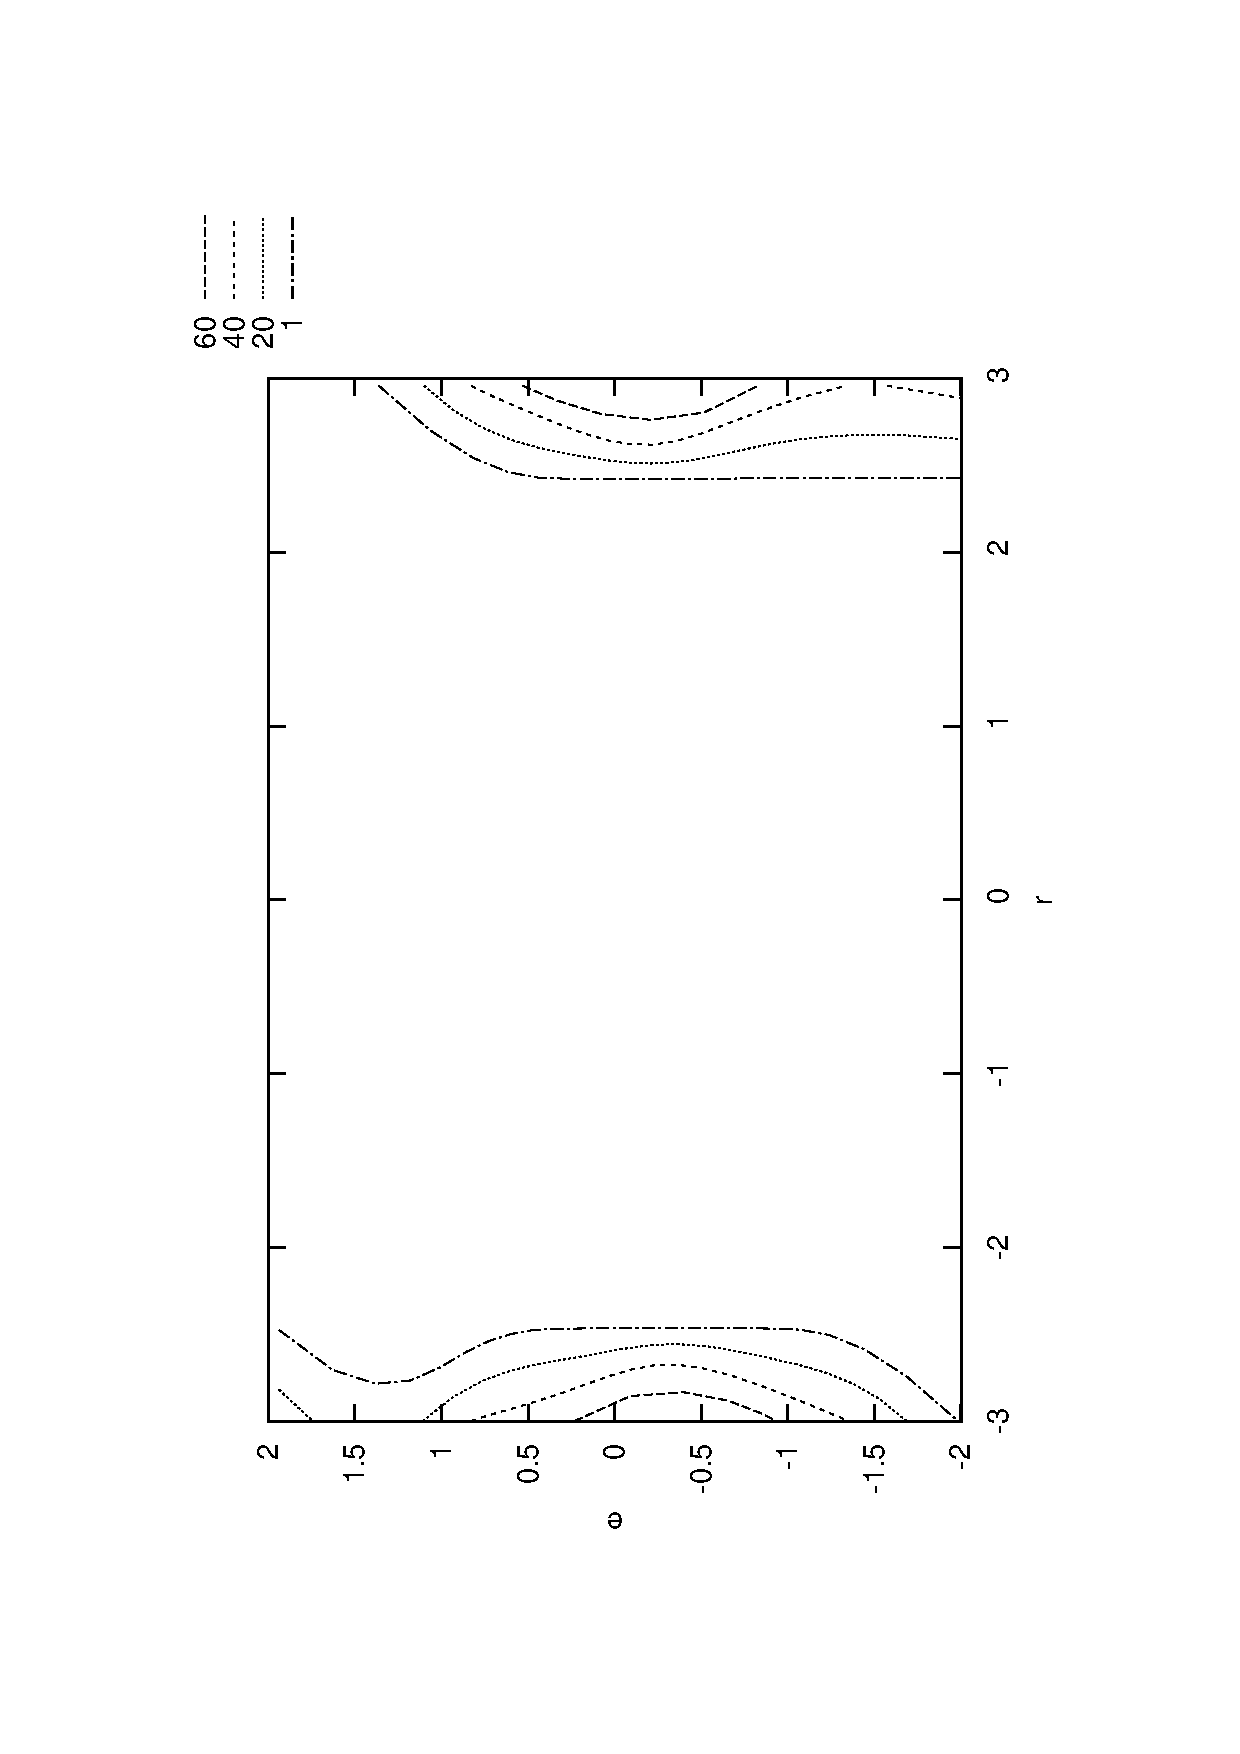
\includegraphics[angle=270,width=0.6\textwidth,%
  totalheight=0.25\textheight]{step_re2d}\\
а)\\
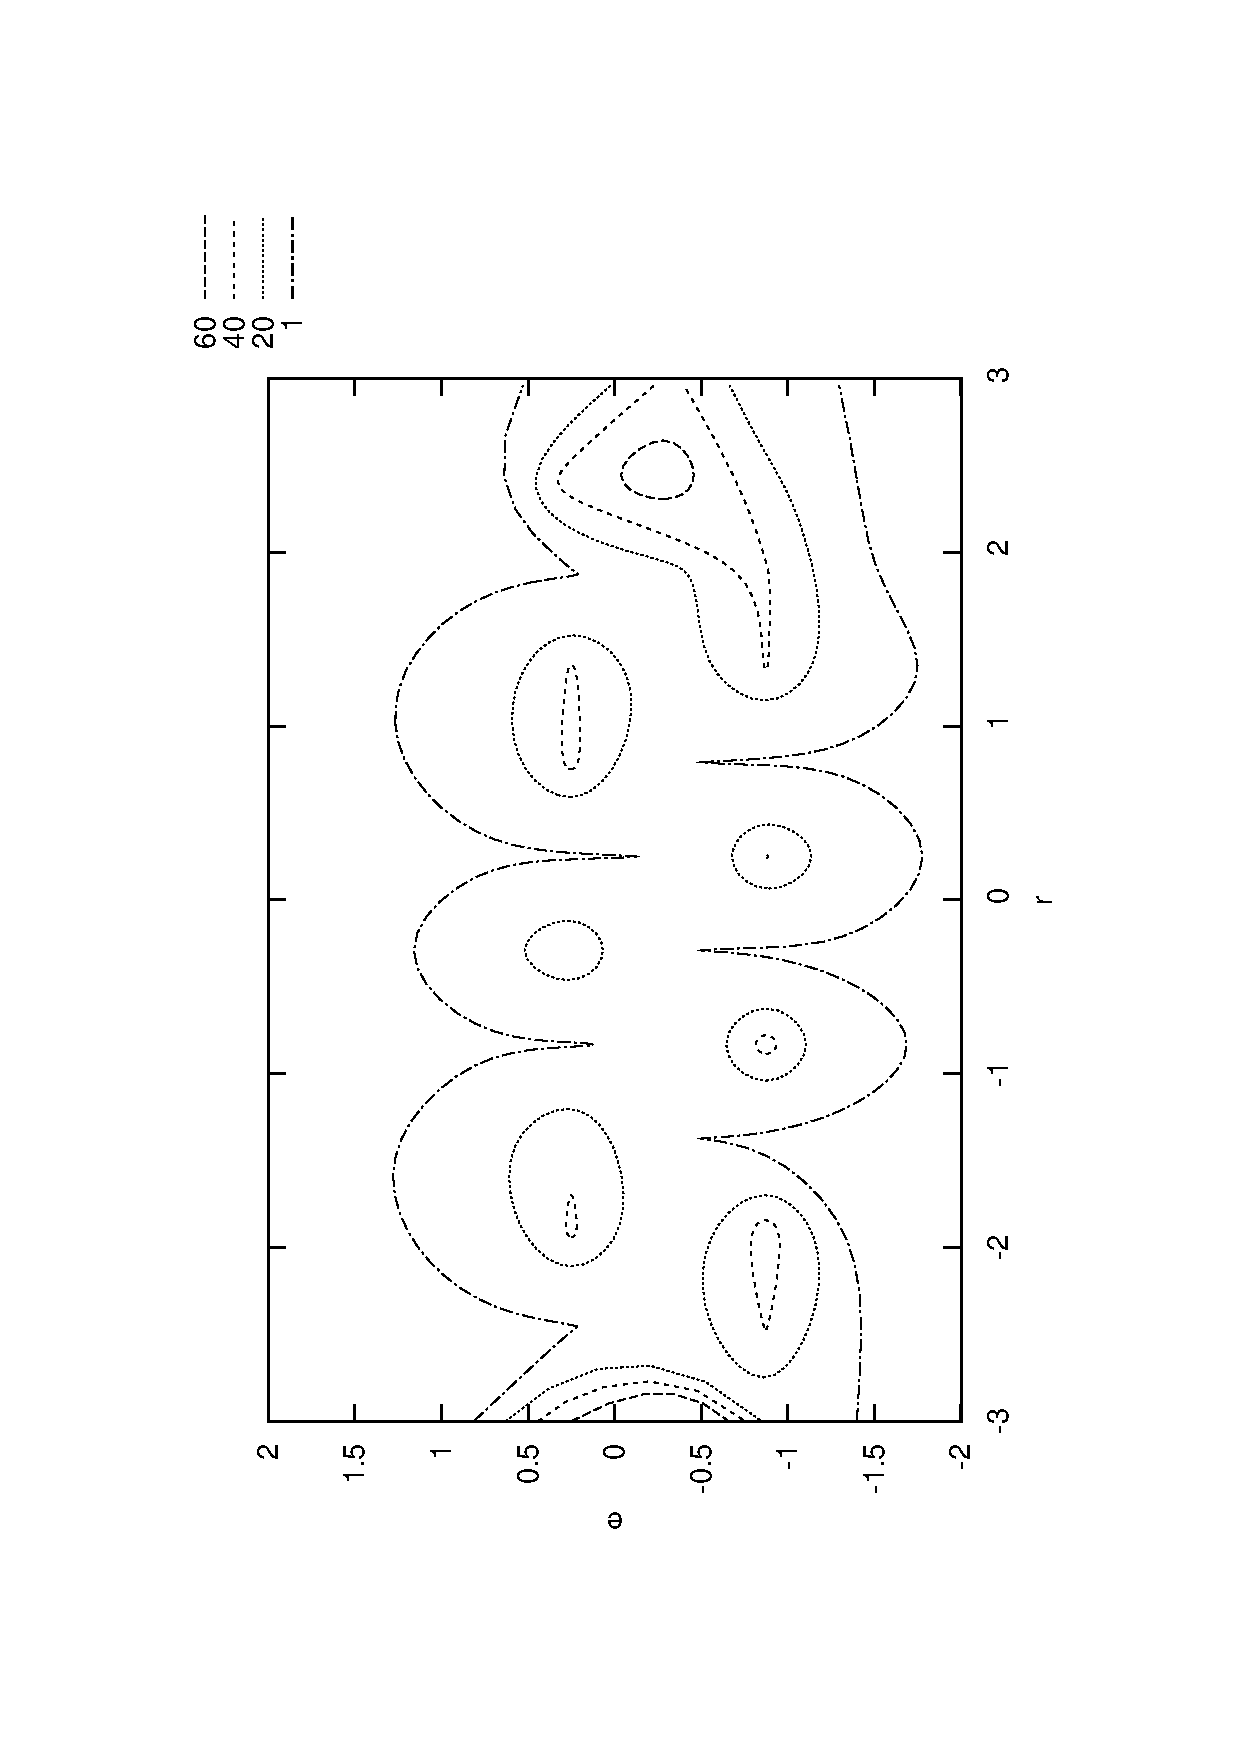
\includegraphics[angle=270,width=0.6\textwidth,%
  totalheight=0.25\textheight]{harm_re2d}\\
б)\\
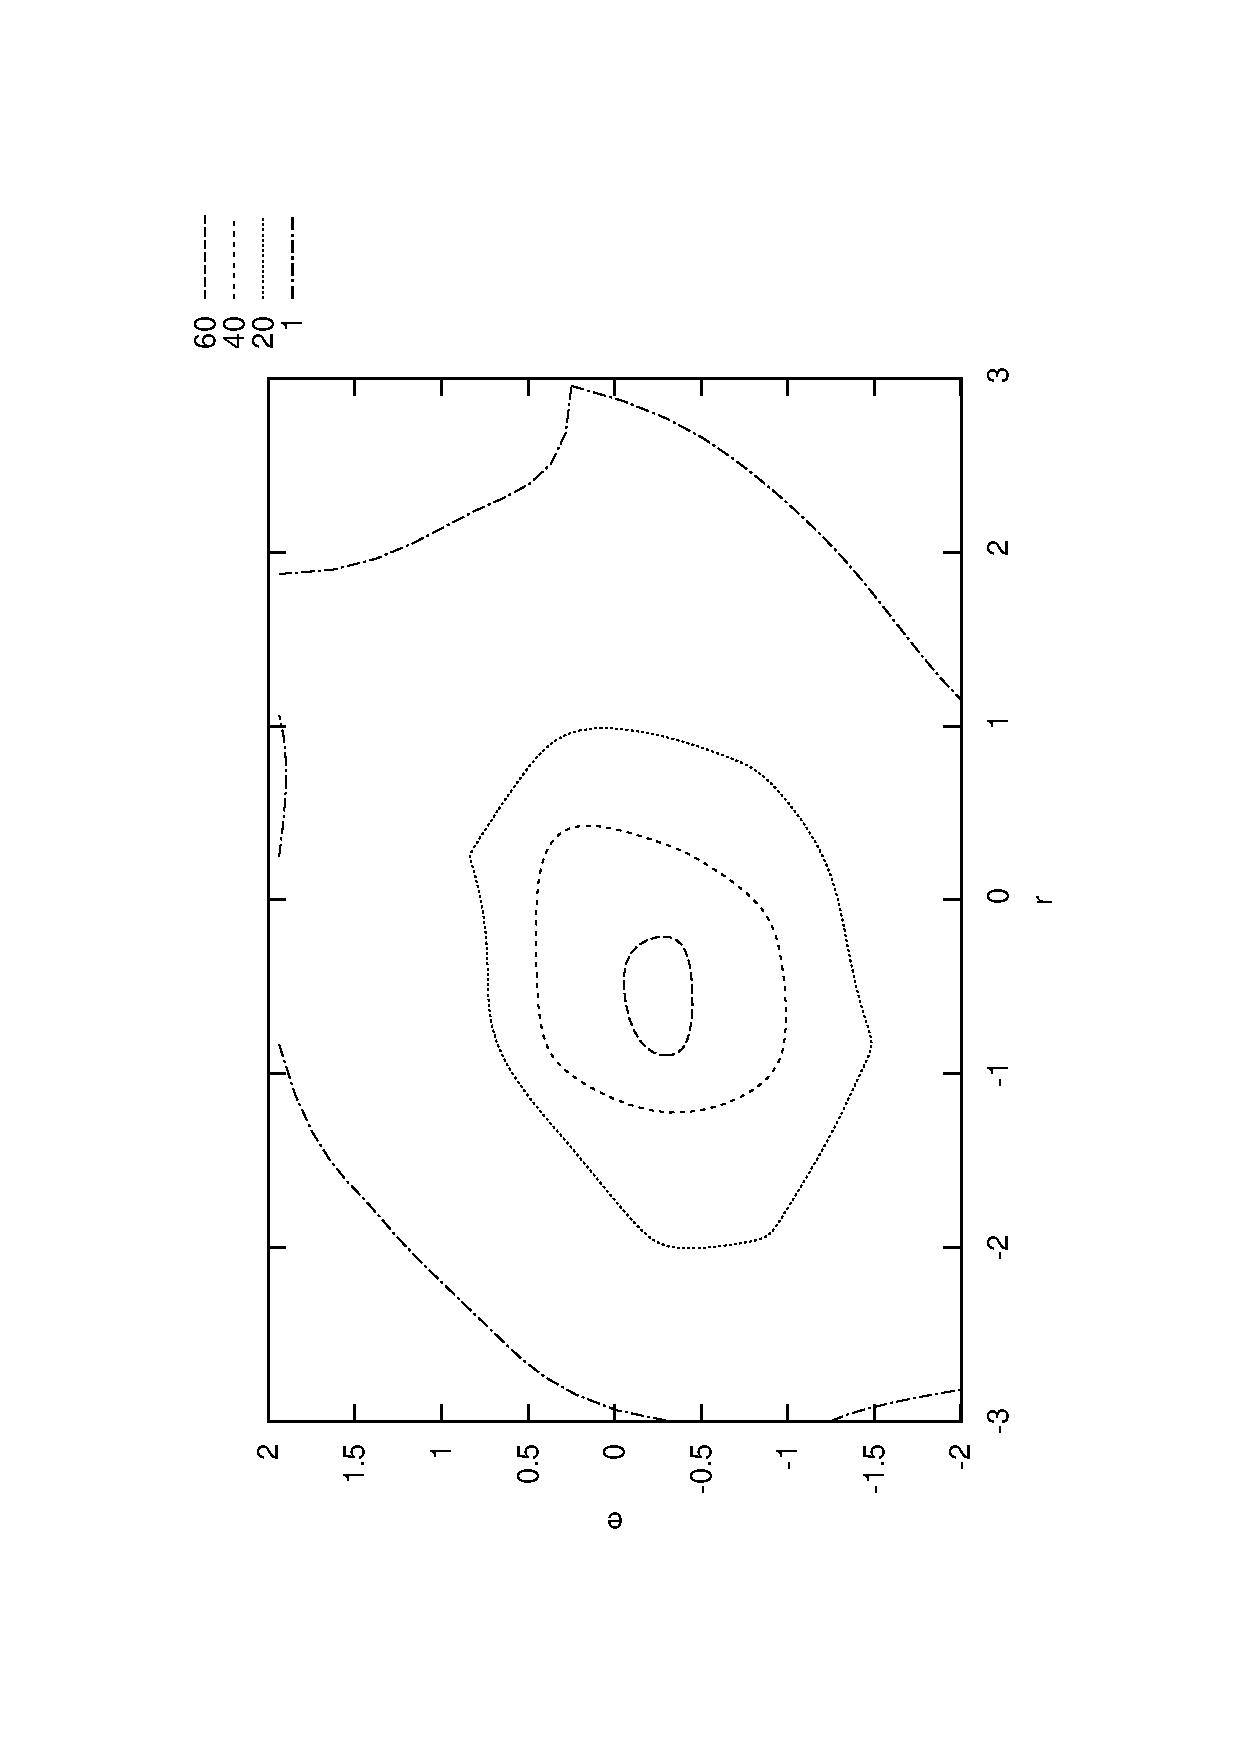
\includegraphics[angle=270,width=0.6\textwidth,%
  totalheight=0.25\textheight]{stoch_re2d}\\
в)\\
\end{tabular}
\caption{Распределение обучающих точек на плоскости $r\times e$
         при ступенчатой периодической (а), моногармонической (б) и
         стохастической уставке (в).}%
\label{fig:probe_signals_re2d}
\end{figure}

Для обозначения границ, в пределах которых нейронная сеть
функционирует с эффективностью, полученной при обучении удобно ввести
термин --- {\em область гарантированного качества}.  Данное понятие
легко конкретизируется на случай обучения нейросетевого регулятора:
если для системы управления известны диапазоны допустимых (или
возможных) уставки и ошибки управления, область гарантированного
качества НС--Р должна охватывать как можно большую часть этих
диапазонов.  Для обеспечения этого требования множество обучающих
данных, полученных на исходной системе управления, должно покрывать
как можно большую часть рабочих диапазонов уставки и ошибки
управления.

Если рабочие диапазоны не заданы, можно оценить параметры
распределения уставки и ошибки накапливать данные в обучающем
множестве до тех пор, пока наиболее вероятный диапазон значений не
будет заполнен с желаемой плотностью.  Плотность обучающих пар должна
быть тем выше, чем больше нейронов (весовых коэффициентов) имеется в
нейронной сети регулятора.

\section{Методика синтеза}

{\LARGE N/A}

\section{Выводы}

\begin{itemize}

\item Разработана методика замены линейного регулятора на примере ПИД
  на нейросетевой.  Эта методика также может применяться и для других
  видов регуляторов, так как предположение линейности исходного
  регулятора нигде не используется явно.

\item Исследован вопрос выбора набора входов для нейросетевого
  регулятора.  Для случая переменной уставки предложено использование
  входов $r_k,e_k$, представляющее собой комбинированный подход к
  управлению по возмущению и отклонению.  Данный выбор обоснован
  результатами вычислительных экспериментов.

\item Для имитации ПИД регулятора обосновано применение простых
  двухслойных персептронов с нелинейными нейронами.

\item Предложена методика рационального формирования обучающей
  выборки.  Для её получения исследованы разные типы пробных сигналов
  и выявлен наилучший --- стохастический.

%TODO
%\item Если будет систематическое сравнение регуляторов, то тут добавить


\end{itemize}
